\subsection{The Gradient \& C-Level Curves}
\noindent
Let $\vec{r}(t)$ be the C-level curve of $f(x, y)$.
\begin{align*}
f\circ\vec{r} &= C  \text{ and } \frac{\mathrm{d}}{\mathrm{d}t}(f\circ\vec{r}) = 0 \\
	&\implies \frac{\mathrm{d}}{\mathrm{d}t}(f\circ\vec{r}) = \nabla f\cdot\vec{r^\prime}(t) = 0 \\
	&\implies \nabla f\perp\vec{r^\prime}(t) \\
	&\implies \nabla f \text{ is perpendicular to the C-level curve of } f.
\end{align*}

\begin{figure}[H]
	\centering
	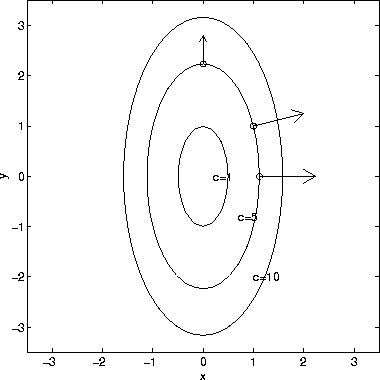
\includegraphics[width=0.33\textwidth]{./differentialMultivariableCalculus/grad_c_level.png}
	\caption{The gradient is perpendicular to C-level curves.}
\end{figure}